%
% appendix.tex
% Copyright (C) 2021 by Krish Kabra, <krish@kabra.com>.
%

\chapter{Deployment Cost Projections for Telemedicine}
\label{chap:telemedicine_cost_projections}

\begin{figure}
    \centering
    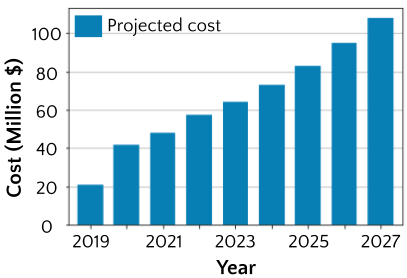
\includegraphics[height=3in]{include/project_costs_fig.png}
    \caption{\textbf{Projected cost of deploying finger pulse oximeters for telemedicine application.} HR sensing solutions for telemedicine and remote patient monitoring have relied on the adoption of wearable sensors. Currently, the most viable and inexpensive existing wearable solution to assess patient HR and oxygen saturation are finger pulse oximeters. For the scales at which telemedicine is projected to grow, such a solution would involve a deployment cost in excess of \$700 million in the US alone. In contrast, a smartphone camera-based method offers a purely algorithmic solution that can be integrated into existing healthcare system telemedicine video-conferencing applications.}
    \label{fig:projected_costs_pulseox}
\end{figure}

In order to calculate the estimated average deployment cost for the cheapest existing method (finger pulse oximeters), we use the following methodology:
\begin{enumerate}
    \item We identify the estimated user base numbers for telemedicine in the US using the numbers from \cite{kats_us_2020} and extend these up to 2027 using the compound annual growth rate (CAGR) of 15.8\% as suggested in \cite{polaris_us_2020}.
    
    \item We make the conservative assumption that all members of a given family would be active users of telemedicine services. Therefore, an estimate of the number of families using telemedicine services is given by: 
    \begin{equation}
        No.~of~Families = \frac{Number~of~Telemedicine~Users}{Avg.~Family~Size~in~the~US}
    \end{equation}
    We use the average family size of 3.15 from the U.S. Census Bureau's Current Population Survey \cite{cps_us_2020}.
    
    \item Assuming that one pulse oximeter costs \$20 (as observed from a survey of available units in the market), and assuming conservatively that one pulse oximeter has to be deployed per family, the cost of deployment is given by: 
    \begin{equation}
        Cost~of~Deployment = No.~of~Families~\times~Cost~per~Pulse~Oximeter~Unit
    \end{equation}
\end{enumerate}





